\chapter{Solution}

\section{Hardware}
% Responsible: Lukas Krahbichler

\subsection{Computer}

Several single-board computers were evaluated for this project:

\begin{itemize}
	\item \textbf{NVIDIA Jetson Nano:} Offers strong AI capabilities but is more expensive and exceeds project requirements \cite{nvidia_jetson_nano}.
	\item \textbf{ASUS Tinker Board S:} Affordable but lacks sufficient computational power for real-time image processing \cite{asus_tinkerboard_s}.
	\item \textbf{ArmSom Sige7 (Basic):} Balances affordability and performance, supporting necessary image processing tasks \cite{armsom_sige7}.
	\item \textbf{Raspberry Pi 4 Model B (8GB):} Well-supported but has less processing power for image processing compared to other options \cite{raspberry_pi_4b}.
\end{itemize}

The ArmSom Sige7 Basic \cite{armsom_sige7}, equipped with a Sige Active Cooling Kit \cite{armsom_sige_cooling_kit}, was chosen for its adequate performance and cost-effectiveness. However, during development, issues arose: one of the three units failed to boot, and limited documentation and support made troubleshooting difficult. In hindsight, selecting a more widely adopted platform like NVIDIA, ASUS, or Raspberry Pi would have offered greater reliability and community support.

In the end, this hardware failure was one of the main reasons the project was not fully completed, along with time constraints that prevented further troubleshooting or contacting the manufacturer, and the high costs associated with hardware replacement.

\subsection{Camera}

The camera module chosen was the 4K model from ArmSom \cite{armsom_camera_module}, specifically designed for seamless integration with the ArmSom Sige7 \cite{armsom_sige7}. This ensured full hardware compatibility and eliminated potential issues with third-party components. The module was selected for its high resolution, which allows for better tracking accuracy at greater distances. However, during testing, the camera initially produced very dark images. This was traced back to a driver issue, which was quickly resolved with support from the manufacturer.

\subsection{Display}

Initially, a 10.1-inch Full HD display from ArmSom \cite{armsom_display} was integrated into the primary station. The display was chosen for its compatibility with the ArmSom Sige7 \cite{armsom_sige7} and its reasonable price. However, as the project progressed, a redesign of the housing necessitated its removal. Redirecting the visualization to a laptop allowed for a more compact and efficient housing design.

\subsection{Power Supply}

The chosen power supply was a PD 100 W, 20,000mAh power bank from POWERADD PRO \cite{poweradd_pro_powerbank}. This model met the project's technical requirements as follows:
\begin{itemize}
	\item It supports USB-PD, essential for powering the ArmSom Sige7 \cite{armsom_sige7}.
	\item Its 100W output ensures compatibility with all connected components, including the \acrshort{pcb}.
	\item It has three ports, enabling simultaneous connections for the ArmSom board, the \acrshort{pcb}, and charging functionality.
\end{itemize}

Despite meeting these specifications, several issues arose during use. The power bank exhibited unpredictable behavior, intermittently cycling on and off. While this occurred less frequently when the power bank was fully or nearly fully charged, the problem was never completely resolved. Additionally, unexpected voltage drops were observed on the \acrshort{pcb}, with measurements showing 3.6V instead of the expected 5V from the USB output. This raised concerns about power stability and its impact on system reliability. Furthermore, it is highly likely that one of the ArmSom computers failed due to unstable voltage levels or power spikes originating from the power bank, though this could not be definitively confirmed.

Additionally, with this setup, the station has two start buttons: one for the power bank and one for the ArmSom.

\subsection{Data Transfer}

Initially, the NRF24L01 \cite{nRF24L01} modules with \acrshort{pcb} antennas were integrated directly onto the \acrshort{pcb} to enable local radio communication between stations. However, these modules proved unreliable in the required 3-node mesh system, frequently failing to maintain stable communication.

To resolve this, the system was upgraded to NRF24L01+ PA + LNA \cite{nRF24L01_plus} modules with external antennas. This change improved signal strength but required modifications to the housing design to accommodate the larger modules. The \acrshort{pcb} remained unchanged due to the identical pinout, but the new modules were too large to be mounted directly. Instead, they had to be repositioned and connected via jumper cables.

During testing, the mesh network continued to exhibit failures or functioned only when antennas were placed in specific orientations. Further research indicated that the high transmission power of the new modules caused interference in close-range operation. Reducing the transmission power resolved these stability issues, allowing the modules to function reliably within the system.

\subsection{Calibration}

The calibration hardware ensures precise alignment and positioning of the primary and secondary stations for 3D tracking. Each station features a rotatable head for pitch and yaw adjustments, while roll is compensated via gyroscope measurements. Secondary stations share the same design for simplicity, but only the primary station includes a Time-of-Flight (ToF) laser for precise distance measurement. Secondary stations rely on camera-based alignment.

\subsubsection*{Components and Functionality}

\paragraph{Rotatable Head (Pitch and Yaw Axes):}
The system uses compact 28BYJ-48 stepper motors controlled via ULN2003 driver boards \cite{angeek_28byj_48}. End-switches from InduSKY \cite{indusky_microswitch}, configured in normally closed mode, detect faults like loose connections. Servos \cite{miuzei_servos} were initially considered but dismissed due to cost, size, and complexity.

\paragraph{Gyroscope and Compass:}

Initially, we attempted to use a \textbf{9DOF sensor module} \citep{jwbl_dof_sensor} that integrated a 3-axis 12-bit accelerometer, a 3-axis earth magnet sensor, and a 3-axis 16-bit gyroscope. However, the gyroscope did not function at all, while the accelerometer and magnetometer failed to provide correct data. The earth magnet sensor, in particular, delivered inconsistent readings, fluctuating significantly between measurements and rendering it unreliable for absolute orientation.

As a result, we switched to a \textbf{GY-521 gyroscope} \cite{azdelivery_gy_521}, which provides 6-axis data for tilt measurement and alignment correction. Additionally, a \textbf{GY-271 compass} \cite{azdelivery_gy_271} was initially included for absolute orientation but was later abandoned due to unreliable calibration and inconsistent results. The compass remains on the \acrshort{pcb} but is not actively used in the system.

\paragraph{ToF Laser Module:}
The primary station features a DFRobot Infrared Laser Distance Sensor \cite{dfrobot_ir_sensor} with a 5 cm to 80 m range and millimeter-level accuracy. It is used for precise distance measurements and requires an unobstructed line of sight between the stations.

\paragraph{Camera for Visual Alignment:}
Each station’s 4K camera \cite{armsom_camera_module} identifies and aligns with other stations during calibration. The cameras should track the bright orange secondary stations for positioning, replacing the originally planned but unreliable radio-based direction-finding approach with LoRa-Modules \cite{tecnoio_lora_modules}.

\paragraph{Calibration \acrshort{pcb}:}
The calibration system relies on a custom-designed \acrshort{pcb} to integrate various components necessary for precise positioning and alignment. The \acrshort{pcb} was designed using \textbf{Altium Designer 22} \cite{altium_designer_22}, with components sourced from \textbf{DigiKey} \cite{digikey} and the board itself manufactured by \textbf{JLCPCB} \cite{jlcpcb}. Assembly was completed both in the school’s workshop and at home, with components manually soldered.

The \acrshort{pcb} incorporates an \textbf{Arduino Nano} manufactured by DFRobot \cite{arduino_nano_dfrobot} as the main microcontroller. However, during development, we encountered program storage limitations, restricting the complexity of the firmware. In hindsight, selecting a microcontroller with more program storage, such as the \textbf{Arduino Uno}, would have provided more flexibility and prevented these constraints.

\textbf{Key Functions of the \acrshort{pcb}:}
\begin{itemize}
	\item Provides power distribution to the calibration components.
	\item Interfaces with the stepper motor drivers for head rotation control.
	\item Integrates the gyroscope, compass, and ToF laser module.
	\item Facilitates LED indicators for status feedback.
\end{itemize}

\textbf{Issues Encountered During Development:}
\begin{itemize}
	\item The \textbf{USB input connector} was never soldered because the cable would not fit inside the housing. Instead, wires were directly soldered to the board.
	\item The \textbf{Arduino orientation} was incorrect in the Altium design, resulting in the microcontroller being mounted in the opposite direction than originally planned. This led to changes in cable management in the housing design.
	\item The \textbf{LED on/off switching functionality} did not work as intended, requiring two additional manual connections to be made on each \acrshort{pcb}.
	\item The \textbf{Communication between the Arduino Nano \cite{arduino_nano_dfrobot} and the ArmSom Sige7 \cite{armsom_sige7}} was initially planned via I2C. However, this did not work as expected. After unsuccessful troubleshooting attempts, we switched to UART communication. This change caused issues with the camera, as both systems could not run simultaneously. Ultimately, we resolved this by using a direct USB connection, running a cable from a USB-A port on the ArmSom board to the Micro-USB port on the Arduino Nano.
\end{itemize}

Despite these issues, the \acrshort{pcb} successfully serves as the central interface for calibration hardware, integrating all necessary sensors and controllers to facilitate the calibration process.

\subsubsection*{Calibration Hardware Conclusion}
While the calibration system was designed to reduce costs compared to \acrshort{gnss} with \acrshort{rtk}, the final implementation became expensive. In hindsight, the cost was close to that of \acrshort{rtk}-based alternatives used by competitors.

\section{Housing}
\subsection{First Version}  

The initial housing design was developed before all hardware components were physically available, relying exclusively on online specifications and manufacturer-provided measurements. While this approach enabled early prototyping, it also introduced dimensional inaccuracies. One of the most notable issues was an incorrectly sized display cutout, which required significant adjustments and a complete reprint of the housing.  

As the project progressed, multiple redesigns became necessary to refine the housing’s functionality and accommodate unforeseen challenges.

\paragraph{Adaptation to Hardware Changes}  
As final hardware selections were made, modifications were required to ensure a proper fit for all components. Throughout the development process, some components were replaced or upgraded, necessitating corresponding adjustments to the housing design. This iterative approach ensured compatibility with the latest hardware configurations while maintaining structural integrity.  

\paragraph{Improved Accessibility}  
To facilitate maintenance and future modifications, internal components needed to be more easily accessible. Several design refinements were implemented, including repositioning mounting points, enlarging access openings for connectors, and improving ventilation. These changes simplified servicing and upgrades, reducing downtime and enhancing long-term usability.  

\paragraph{Simplified Assembly and Structural Refinements}  
Initial prototypes were complex and time-consuming to assemble. To address this, the design was incrementally refined to minimize the number of assembly steps and reduce the likelihood of errors. Additionally, the housing was structured as a modular system, consisting of multiple interlocking parts. This approach optimized printability within standard 3D printing constraints while also enhancing maintainability, as individual sections could be replaced or upgraded without requiring a complete reprint.  

\paragraph{Key Design Challenges and Iterative Improvements}  
Throughout development, several specific design challenges emerged, necessitating further refinements:  
\begin{itemize}  
	\item \textbf{Countersinks:} Initially too small, requiring adjustments based on print quality to ensure proper screw seating.  
	\item \textbf{Screw Holes:} Some holes were oversized, allowing screws to spin freely instead of securing properly. This was addressed by refining tolerances for a precise fit.  
	\item \textbf{Tolerance Adjustments:} Various fitment issues arose due to minor dimensional inaccuracies, requiring iterative refinements to achieve optimal compatibility between components.  
	\item \textbf{Ventilation:} Early prototypes lacked sufficient airflow, increasing the risk of overheating. Ventilation openings were expanded and repositioned to enhance cooling efficiency.  
	\item \textbf{Structural Stability:} Additional reinforcements were implemented to ensure that the housing could withstand vibrations and external forces during operation.  
	\item \textbf{Hardware Integration:} Mounting positions were refined to simplify the integration of components, improving ease of assembly and overall usability.  
	\item \textbf{Port Accessibility:} The layout was adjusted to provide better access to the computer’s ports, simplifying connectivity.  
\end{itemize}  

These continuous iterations and refinements allowed the first version of the housing to evolve into a more practical and functional design. The lessons learned from this phase directly influenced subsequent iterations, leading to an optimized final version.  
  
  
\subsection{Second (Final) Version}
Building upon the insights gained from the first housing iteration, the second version introduced several key improvements to enhance functionality, maintainability, and overall design efficiency.  

\paragraph{Enhanced Modularity and Accessibility}  
A major focus of the redesign was to improve modularity, simplifying both assembly and maintenance. The revised structure allows for more efficient disassembly, significantly reducing the time required for maintenance and hardware adjustments. Additionally, hardware accessibility was prioritized, ensuring that critical components could be reached without excessive disassembly.  

\paragraph{Compact and Optimized Design}  
One of the most impactful changes was the removal of the display, which had previously dictated the dimensions of the housing. This adjustment enabled a more compact and streamlined design, optimizing space utilization while maintaining full functionality. Despite these structural changes, the motor mechanism from the first version was retained, reducing development time and ensuring continuity in core functionalities.  

\paragraph{Redesigned Bottom Section}  
The bottom section of the housing, which accommodates essential components such as the \acrshort{pcb}, computer, power bank, and cooling system, underwent a complete redesign. This revision focused on improving organization, airflow, and ease of access to internal hardware, ensuring more efficient operation and maintenance.  

\paragraph{Integration of Threaded Inserts}  
To enhance durability and improve the reliability of screw connections, threaded inserts were introduced. These additions provide several benefits:  
\begin{itemize}  
	\item Increased longevity of screw mounts, preventing wear and deformation over multiple assembly cycles.  
	\item Simplified disassembly and reassembly, facilitating faster maintenance and upgrades.  
	\item Enhanced structural integrity, ensuring that fastening points remain secure over time.  
\end{itemize}  

\paragraph{Yaw Motor Issue \& Gear System Upgrade}  
During testing, the initial yaw motor was found to be underpowered, resulting in performance limitations. To address this issue, a gear system was implemented to increase torque, enabling smoother and more reliable movement. This upgrade ensured that the system could operate effectively under varying conditions without compromising precision or stability.  

\paragraph{Refinements to the Bottom Section}  
Even after the major redesign, additional modifications were necessary to further optimize the housing’s performance and durability:  
\begin{itemize}  
	\item Improved interconnections between housing parts, enhancing structural integrity.  
	\item Optimized airflow channels to improve cooling efficiency and prevent overheating.  
	\item Increased overall stability to withstand vibrations and external forces.  
	\item Adjusted hardware mounting positions for seamless integration and accessibility.  
	\item Enhanced access to the computer’s ports, ensuring convenient connectivity.  
	\item Redesigned power button mechanism for a more intuitive and reliable user interface.  
\end{itemize}  

By incorporating these refinements, the second housing version achieved a significant leap in reliability, ease of use, and long-term maintainability, making it better suited for real-world deployment.  

\subsection{3D Printing Process}  

The housing components were fabricated using a \textbf{Bambu Lab P1S} 3D printer, chosen for its high-speed printing capabilities and reliable output quality. The material selection varied throughout the development phase to balance rapid prototyping needs with long-term durability requirements.  

\paragraph{Prototyping with PLA}  
During the initial prototyping stage, \textbf{PLA} was used due to its ease of printing and fast turnaround time. This enabled rapid iteration and testing of design modifications without significant material costs. However, PLA's mechanical properties and limited environmental resistance made it unsuitable for the final application.  

\paragraph{Final Production with PETG}  
For the final version, \textbf{PETG} was selected due to its superior durability, higher temperature resistance, and suitability for outdoor conditions. Unlike PLA, PETG offers improved impact resistance and reduced brittleness, ensuring a more robust enclosure for long-term use.  

\paragraph{Considerations for Printing with PETG}  
Although PETG generally requires longer print times and careful tuning compared to PLA, the use of \textbf{High-Flow (HF)} filament allowed for efficient production without a significant increase in cost or time. To ensure optimal print quality, PETG filament was dried for \textbf{eight hours} in a filament dryer before printing. This step was necessary to prevent moisture absorption, which can negatively impact layer adhesion and overall print strength.  

By leveraging the strengths of both materials at different development stages, the housing design was iteratively refined while maintaining efficiency in the fabrication process.

% Responsible: Prantl Niclas

\section{Programming}
\subsection{Development Environment}  

To facilitate efficient and consistent development of the Armsom codebase, a \textbf{custom development environment} was created. This environment builds upon and extends the previously developed system by French Bakery \cite{fb_dev_environment}, incorporating various improvements to enhance usability, maintainability, and cross-platform compatibility.  

\paragraph{Containerized Development Approach}  
A \textbf{Debian-based development container} was employed to provide a standardized environment for \textbf{C++ development and cross-compilation}. By using containerization, all necessary dependencies, libraries, and toolchains are encapsulated within a controlled environment, ensuring that every developer operates under identical conditions, regardless of the underlying host system.  

\paragraph{Cross-Platform Consistency}  
One of the primary motivations for adopting a containerized approach was the need to support development across multiple systems, each running different operating systems. Without a uniform environment, discrepancies in library versions, compiler behavior, and system dependencies could introduce inconsistencies, leading to potential compatibility issues. By utilizing a \textbf{Debian-based development container}, the project ensures:  
\begin{itemize}  
	\item \textbf{Improved Repeatability:} Code behaves identically across all development machines, eliminating system-dependent discrepancies.  
	\item \textbf{Stable and Predictable Development Workflow:} Developers can work with a predefined toolset, reducing setup time and potential conflicts.  
	\item \textbf{Seamless Cross-Compiling:} The containerized approach streamlines cross-compilation, allowing code to be developed on one system while being compiled for another target architecture.  
\end{itemize}  

By leveraging this structured development environment, the project benefits from enhanced collaboration, reduced debugging overhead, and a more streamlined deployment process. This approach not only improves efficiency but also ensures long-term maintainability and scalability of the development workflow.  

\subsection{Hardware Drivers}
A significant portion of the software development effort was dedicated to implementing robust and efficient hardware drivers. These drivers facilitate seamless communication between various hardware components and ensure reliable operation of the system. The hardware control is primarily divided between two processing units: the \textbf{Armsom} (main computer) and the \textbf{Arduino Nano}, each responsible for different aspects of device management.

\begin{itemize}
	\item \textbf{Armsom (Main Computer)}
	\begin{itemize}
		\item Stepper motor drivers
		\item Serial communication with Arduino Nano
	\end{itemize}
	\item \textbf{Arduino Nano}
	\begin{itemize}
		\item RF24 Mesh networking
		\item PWM-based fan control
		\item Time-of-Flight (TOF) laser module
		\item Compass and gyroscope integration
		\item Communication with the Armsom
	\end{itemize}
\end{itemize}

\paragraph{Armsom}
The Armsom is responsible for controlling the stepper motors, ensuring precise movement across both horizontal and vertical axes. A dedicated stepper driver interface provides comprehensive support for various motion parameters, including:
\begin{itemize}
	\item Half-stepping and gear ratio compensation for smooth motion.
	\item Absolute and relative positioning in both steps and angular degrees.
	\item Speed control with acceleration management.
	\item Continuous positional awareness to maintain accurate alignment.
\end{itemize}

To establish a robust communication link with the Arduino Nano, a serial interface was developed, incorporating acknowledgment mechanisms to ensure reliable data transmission. This approach verifies the successful execution of commands and prevents the loss of critical control signals. While the Armsom serves as the central processing unit, it interacts with key hardware components—such as the cooling fan, sensors, and RF24-based networking modules—indirectly through the Arduino Nano, which acts as an intermediary for hardware control and data acquisition.

\paragraph{Arduino Nano}
The Arduino Nano is responsible for handling auxiliary hardware tasks and serves as a bridge between the Armsom and various peripheral components.

\subparagraph{RF24 Mesh Networking}
The RF24 Mesh protocol provides reliable wireless communication between ground stations. The implementation ensures efficient data transfer and message routing across the mesh network. For further details, refer to Section~\ref{subsec:DataTransfer}.

\subparagraph{PWM Fan Control}
A simple pulse-width modulation (PWM) control system is used to regulate the cooling fan speed. The fan is controlled via a single PWM pin, enabling dynamic adjustments based on temperature or other system conditions.

\subparagraph{Time-of-Flight (TOF) Laser}
The TOF laser module is responsible for distance measurements station alignment. A custom serial-based communication interface was developed due to limitations in existing libraries, providing additional functionalities such as:
\begin{itemize}
	\item Checksum validation for data integrity.
	\item Adjustable range and resolution settings.
	\item Laser diode power control (on/off).
	\item Automatic re-request mechanism in case of transmission errors.
\end{itemize}

\subparagraph{Serial Communication with Armsom}
A dedicated serial communication link between the Arduino Nano and the Armsom allows efficient data exchange. Key features of this communication system include:
\begin{itemize}
	\item Buffered message storage for incoming network data until requested by the Armsom.
	\item Memory-efficient design to account for the Nano’s limited RAM capacity.
	\item Integrated debugging capabilities, enabling the Nano to send diagnostic data to the Armsom’s command-line interface (CLI).
\end{itemize}

This modular hardware driver implementation ensures stable, reliable, and maintainable operation across all system components.

%Responsible: Niclas Prantl

\subsection{Calibration}
% Responsible: Lukas Krahbichler

\subsection{Camera Tracking}
% Responsible: Lukas Krahbichler

\newpage
\begin{figure}[H]
	\subsection{Data Transfer} \label{subsec:DataTransfer}
	\centering
	\begin{minipage}{0.5\textwidth} % Text on the left
		\raggedright % Aligns text to the left
		\paragraph{Protocol Overview:}
		
		To ensure reliable and efficient data transmission, a structured JSON-based communication protocol was developed. Each message is encapsulated in a \textbf{parent message}, containing a type, unique ID, and timestamp. The message type can be one of the following:
		
		\begin{itemize}
			\item \textbf{req} – Requests information or an action.
			\item \textbf{ack} – Confirms successful execution of an action.
			\item \textbf{repl} – Provides responses to requests.
			\item \textbf{data} – Transmits tracking or station-related information.
		\end{itemize}
		
		with each message type having a specified schema. In case the message type is \textbf{data}, it can be further separated in:
		
		\begin{itemize}
			\item \textbf{Target Result (tres)}: Contains object tracking data, including camera angles and object IDs.
			\item \textbf{3D Target Result (tres3)}: Extends \textbf{tres} with precise 3D position.
			\item \textbf{Station Information (sinf)}: Provides metadata on ground stations, including position, direction, and camera specifications.
		\end{itemize}
		
		\paragraph{Protocol Advantages:} \
	
		The protocol ensures:
		\begin{itemize}
			\item \textbf{Efficiency}: Predefined schemas enable fast parsing and low-latency communication.
			\item \textbf{Scalability}: The modular design allows for future extensions.
			\item \textbf{Reliability}: The acknowledgment system provides valuable feedback for error handling.
		\end{itemize}
		
		This structured approach enables seamless coordination between ground stations, visualization tools, and tracking algorithms.
		
	\end{minipage}%
	\hfill
	\begin{minipage}{0.38\textwidth} % Image on the right
		\centering
		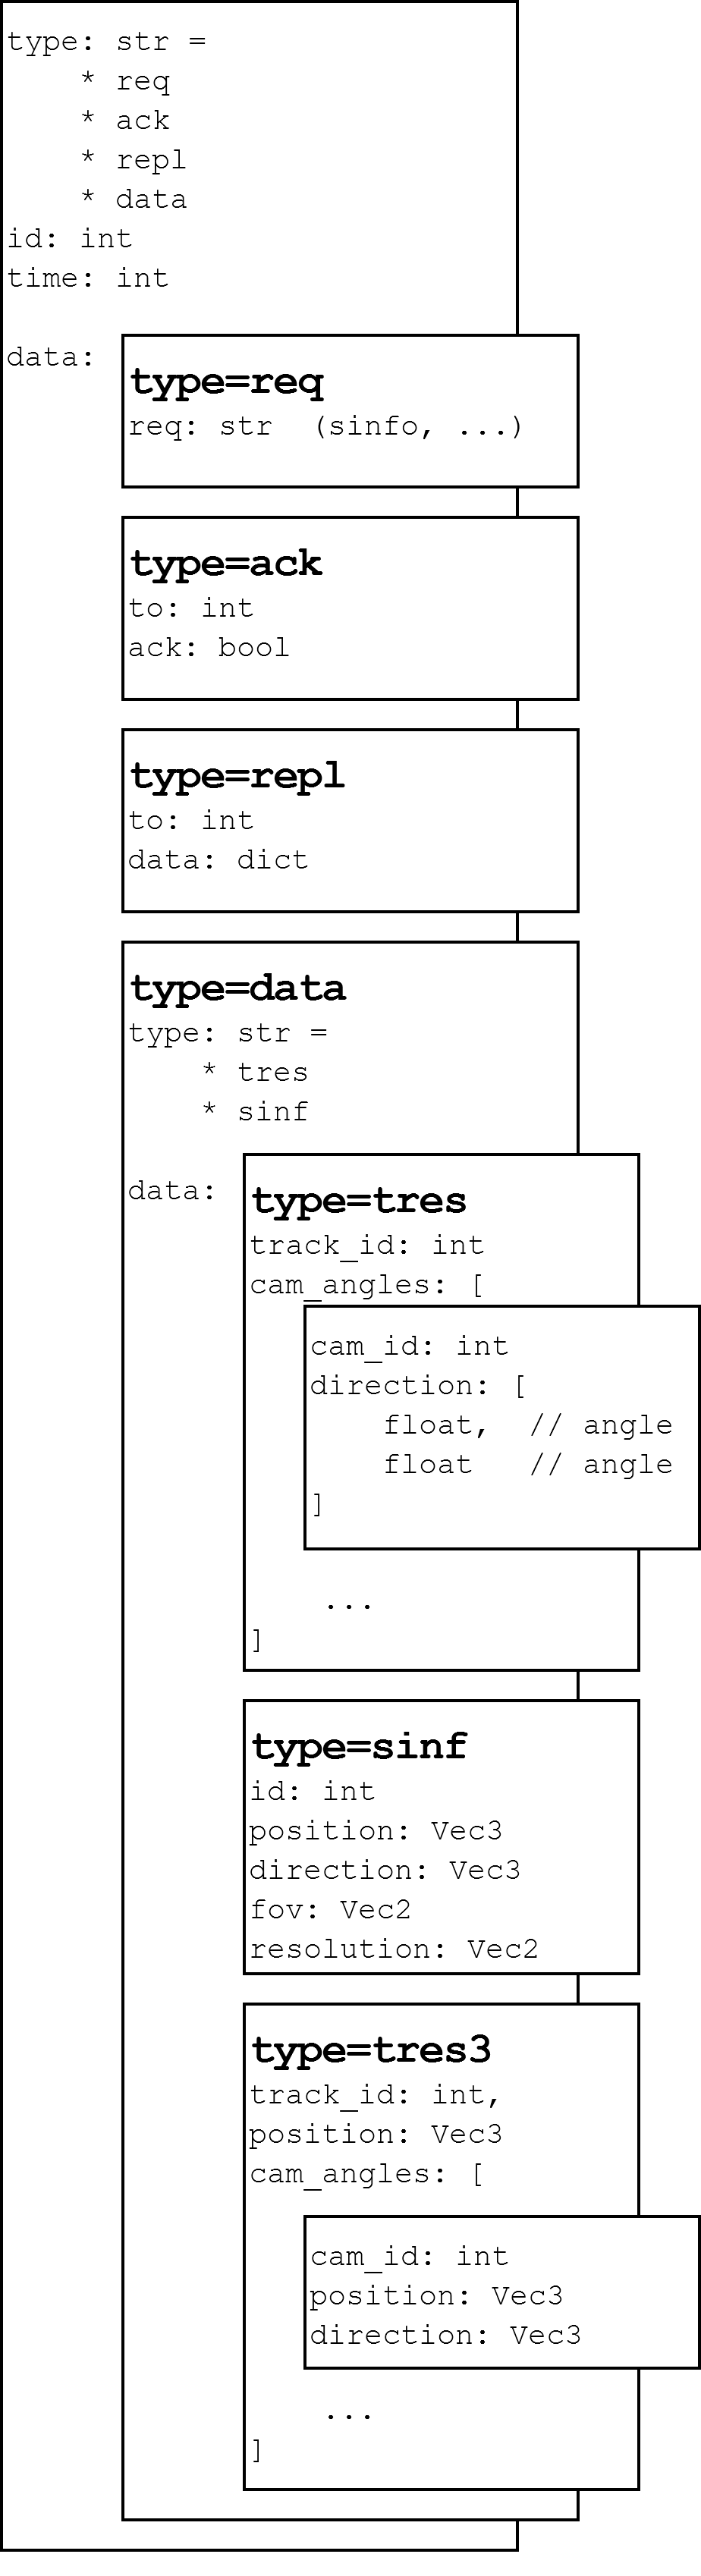
\includegraphics[width=\textwidth]{figures/SS_Protocol_Message}
		\caption{Message Structure}
		\source{Own illustration created with Draw.io}
		\label{fig:ssprotocolmessage}
	\end{minipage}
\end{figure}

\paragraph{Theoretical Solution:}  
To establish a robust and efficient communication framework, all three ground stations are integrated into a \textbf{Mesh network}, where the \textbf{primary station} assumes the role of the central server, while the \textbf{secondary stations} operate as clients.

During system initialization, the primary station enters a \textbf{standby state}, waiting for all secondary stations to establish a connection. Once all connections are confirmed, the system initiates a calibration procedure, synchronizing positional data and aligning reference frames to ensure precise tracking and analysis.  

For standard operation, the primary station transitions into a \textbf{listen-only mode}, except for sending essential acknowledgments. This strategic design significantly reduces computational overhead and minimizes RAM usage, allowing the system to maintain high efficiency even under demanding conditions. By limiting active processing on the primary station, the architecture optimizes real-time data handling while ensuring rapid and reliable communication between all networked components.  

This approach not only enhances the system's scalability but also improves fault tolerance by enabling seamless reconnections in case of temporary communication disruptions.  

\paragraph{Code Implementation:}  
The implementation of the communication framework was significantly streamlined by leveraging the \texttt{RF24Network} and \texttt{RF24Mesh} libraries, which provide a robust abstraction layer for interfacing with the \texttt{NRF24L01+ PA + LNA} modules. These libraries handle much of the low-level networking functionality, including packet routing, automatic retransmissions, and dynamic addressing, thereby reducing development complexity and allowing for a more structured and maintainable architecture.  

However, to fully integrate the system’s requirements, a modular software interface needed to be developed, capable of supporting both \textbf{server} (primary station) and \textbf{client} (secondary station) nodes. This involved designing a flexible communication framework that could dynamically handle various message types, manage connections efficiently, and ensure reliable data transfer.  

A key aspect of the implementation was integrating the previously defined \textbf{custom network protocol}, which structures and organizes all transmitted data. The protocol was designed to handle distinct message types, including requests, replies, acknowledgments, and data transmissions. Within data messages, further categorization enables the transmission of tracking results and station-specific information.  

By adopting this structured approach, the system benefits from improved scalability, reduced processing overhead, and enhanced reliability, making it well-suited for real-time applications with stringent performance requirements.  

% Responsible: Lukas Krahbichler

\subsection{3D Angle Calculations}
\paragraph{Approach:}
In contrary to the initially proposed "simple trigonometry", the calculations are being done using an approximation algorithm. This approach was chosen, because the vectors from each station to the target will never be fully accurate, so in the real world the three Vectors would never meet, which makes solving it using trigonometry impossible. Approximation works, by specifying a "rule set" (a function returning an integer) and trying to achieve the lowest possible output value, using a three dimensional position as input parameter. 

\paragraph{Code Solution:}
In Python, this approximation is performed using \\ \texttt{scipy.optimize.minimize}. The objective function calculates the sum of distances to each line, with lower values indicating points closer to the center of the vector system. The second parameter, \texttt{x0}, defines the starting point for the approximation algorithm, set as the center of our coordinate system, which coincides with the center of our ground station array. Since this function also depends on \texttt{lines}, it must be provided as an argument in \texttt{minimize}. Additionally, the fourth parameter, \texttt{method}, is specified as \texttt{"BFGS"}.

\textbf{Broyden–Fletcher–Goldfarb–Shanno algorithm:} \\
The Broyden–Fletcher–Goldfarb–Shanno (BFGS) algorithm is an iterative method for solving unconstrained nonlinear optimization problems. It preconditions the gradient with curvature information, gradually approximating the Hessian matrix using a generalized secant method. Unlike Newton’s method, BFGS avoids matrix inversion, reducing computational complexity to O(n2)O(n2) instead of O(n3)O(n3). The L-BFGS variant is efficient for large-scale problems, while BFGS-B handles box constraints. Named after Broyden, Fletcher, Goldfarb, and Shanno, it remains widely used in numerical optimization.\citep{BFGS_wiki}

\hspace*{-1.2cm}

\begin{lstlisting}[style=PythonStyle]
lines: list[tuple[np.array, np.array]] = ...


def objective(
	point: np.array,
	lines: list[tuple[np.array, np.array]]
) -> float:
	"""
	calculate the sum of the distances to each line
	"""
	return sum(distance_to_line(
		point, line[0], line[1]
	) for line in lines)


result = minimize(
	objective,
	x0=np.array([0.0, 0.0, 0.0]),
	args=(lines,),
	method='BFGS'
)
\end{lstlisting}

\begin{figure}[H]
	\centering
	\hspace*{-1.5cm} 
	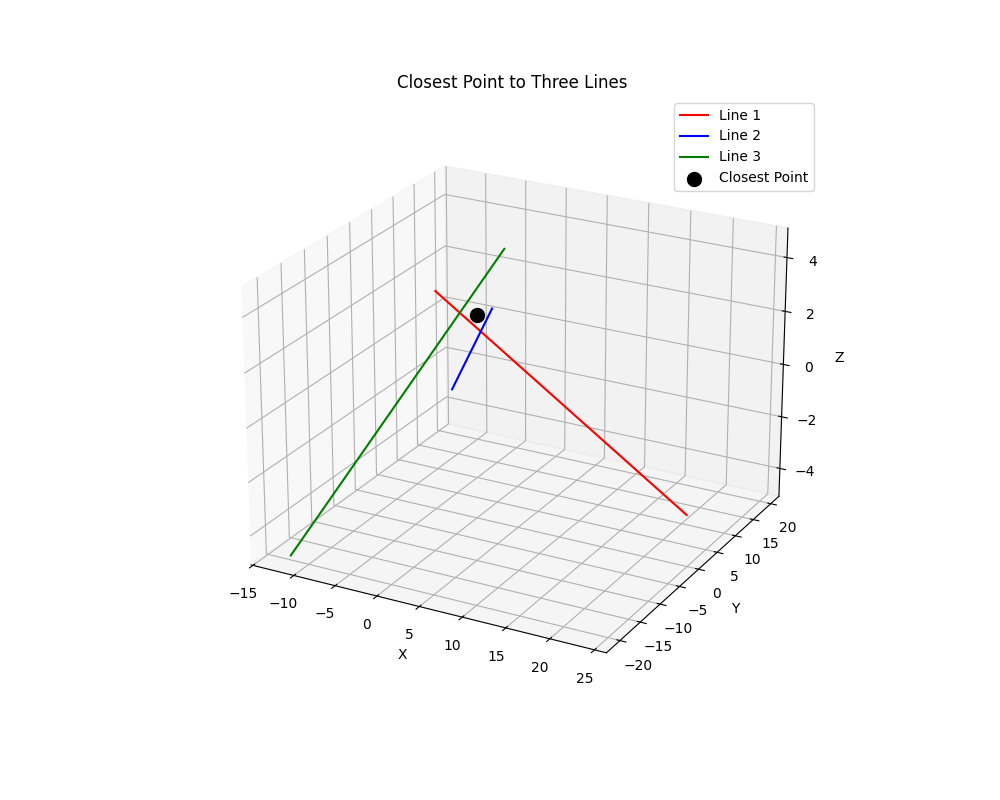
\includegraphics[width=400pt]{figures/approximation_algorithm}
	\caption{Example Visualization of the algorithm}
	\source{Own illustration created with Matplotlib in Python}
	\label{fig:approximationalgorithm}
\end{figure}

As shown in the illustration above, when given three lines in random orientations, the algorithm successfully identifies their center. Testing revealed that the code executes in approximately 400 to 600 µs, which is more than fast enough for our use case.

\paragraph{Tracking}
To enhance target tracking, each identified object is assigned a unique 'track ID,' which allows it to be consistently identified at any given time. Additionally, every calculated position of the object is recorded throughout its movement. This comprehensive data logging makes it possible to fully reconstruct the object's flight path, providing a detailed history of its trajectory and enabling further analysis if needed.

% Responsible: Prantl Niclas

\subsection{3D Visualization}
\paragraph{Network Protocol}  
To ensure broad compatibility and accessibility, the visualization application was designed to run on a wide range of devices, including user-provided hardware. As a result, a dedicated network communication protocol was required to facilitate seamless data exchange between the tracking system and the visualization client.  

To achieve this, the previously defined network protocol was not only reused but also further refined and optimized for this specific application. Unlike a purely request-based system, the server is also capable of broadcasting updates autonomously, ensuring that clients receive critical tracking information in real time. This hybrid approach balances efficiency and responsiveness, allowing visualization clients to both request specific data when needed and passively receive updates without constant polling.  

The refined protocol structure enables the efficient transmission of tracking and calibration data while minimizing network overhead. The updated communication procedure is outlined below:  

\begin{figure}[H]
	\centering
	\hspace*{-1.5cm}
	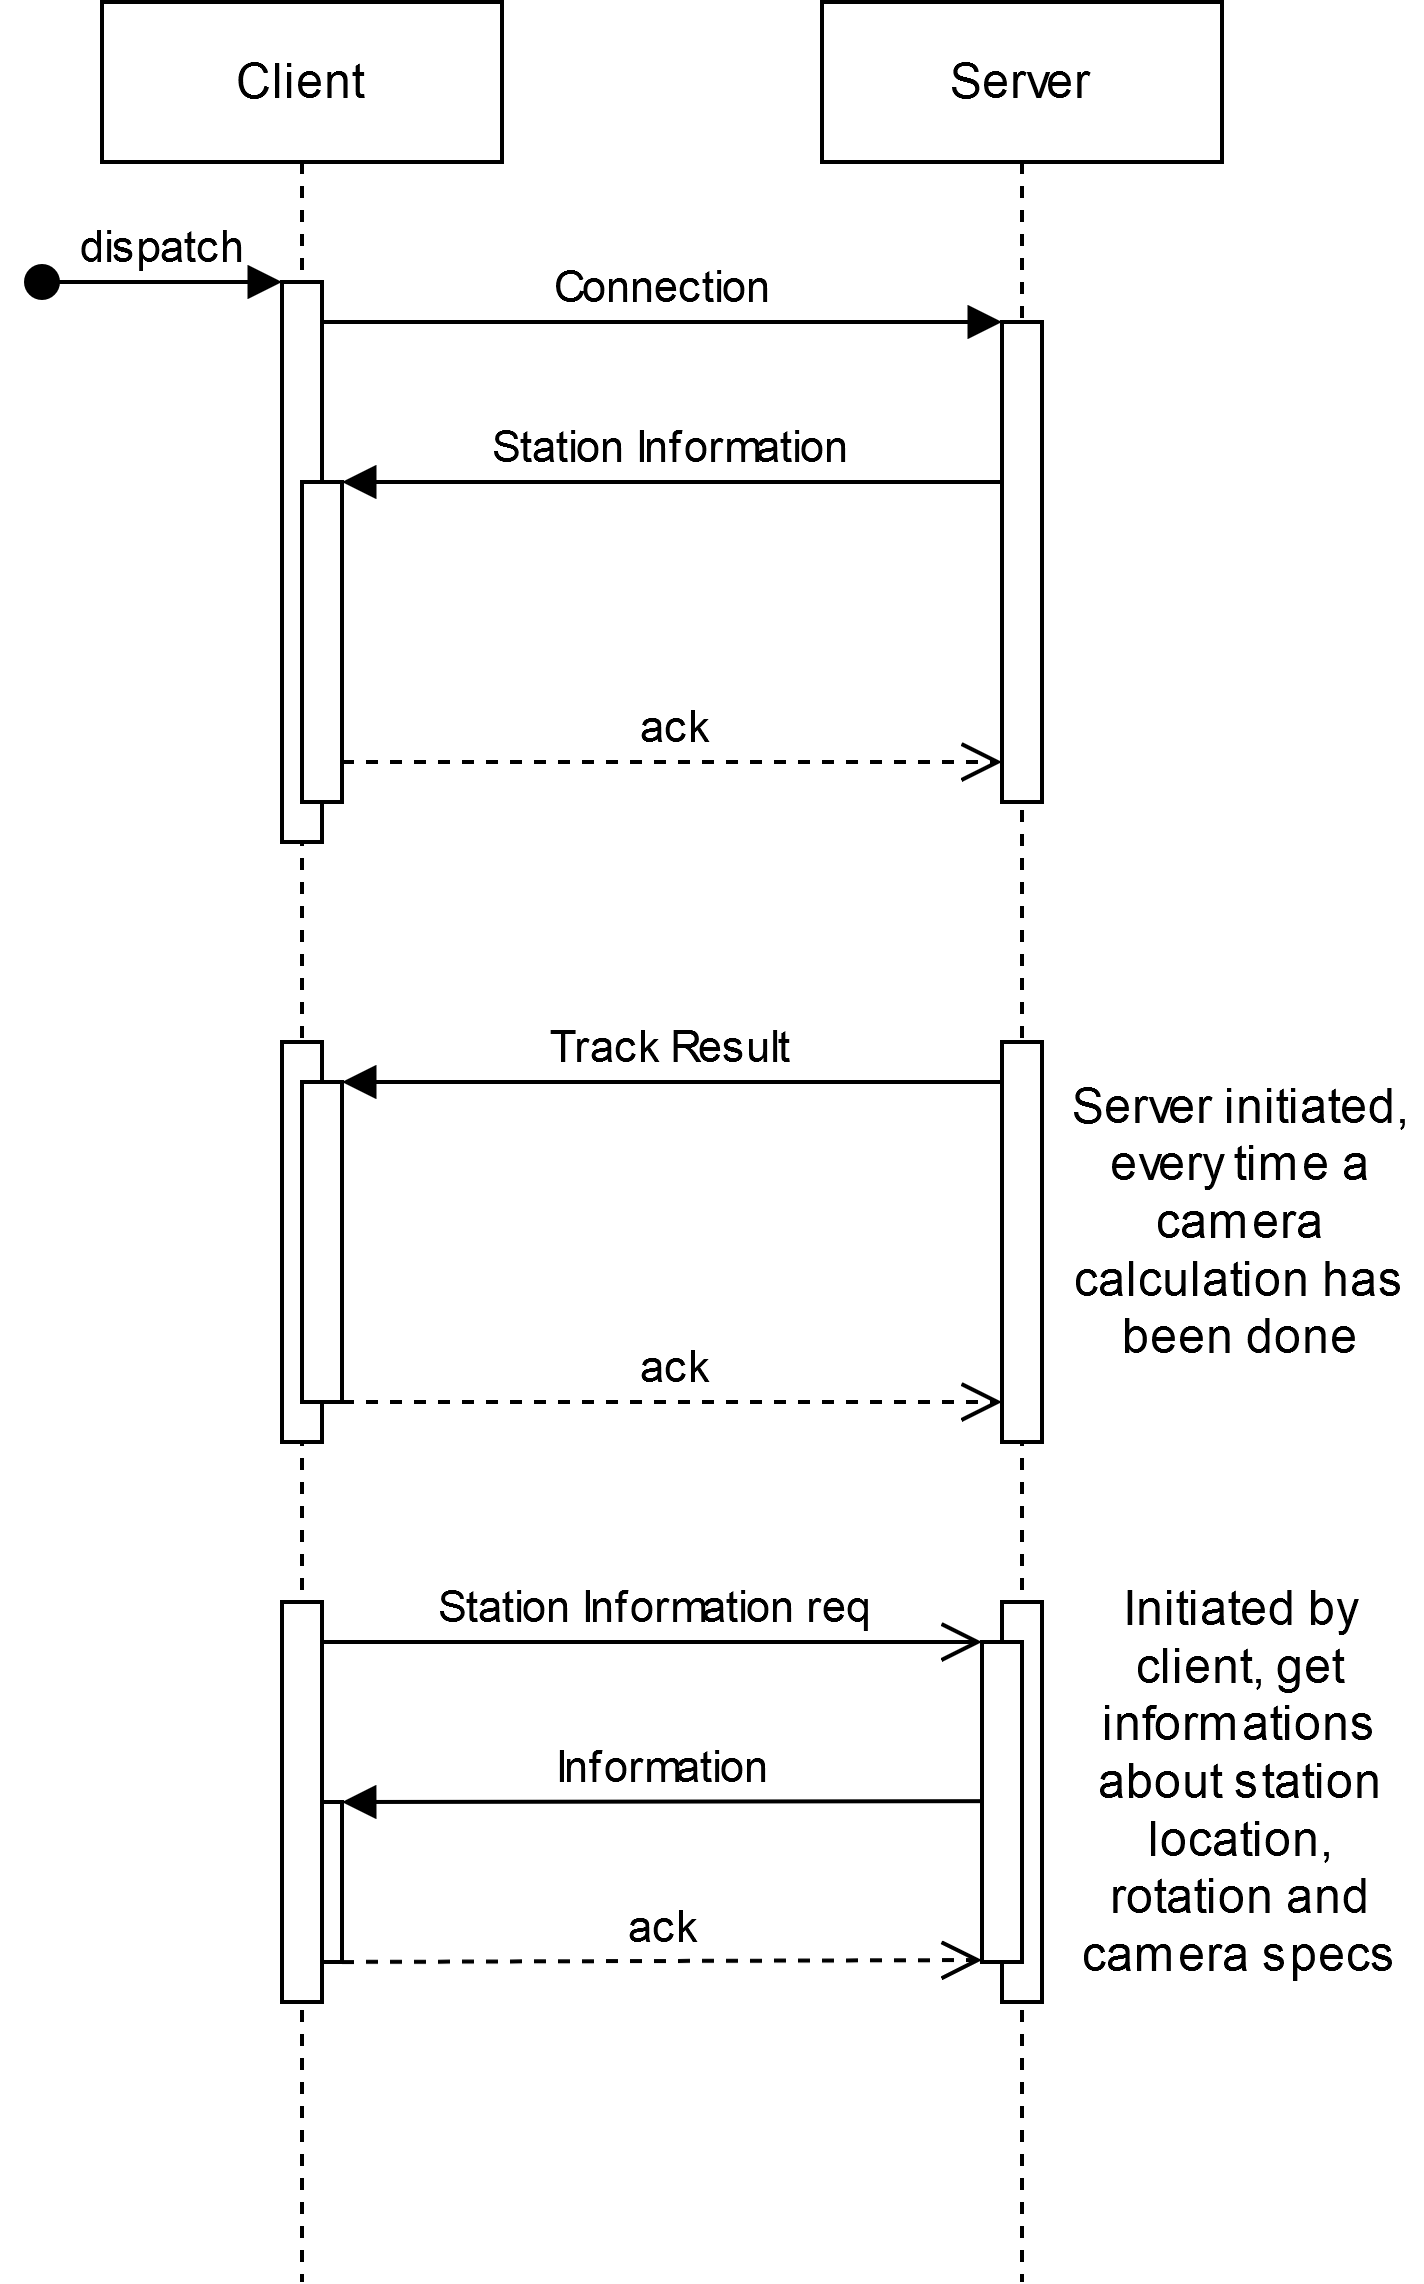
\includegraphics[width=220pt]{figures/SS_Protocol}
	\caption{Simplified Network Protocol}
	\source{Own illustration created with Draw.io}
	\label{fig:ssprotocol}
\end{figure}

\paragraph{Rendering Engine}
Given that the 3D tracking component was already developed in Python, it was a logical decision to implement the visualization system in Python as well to maintain consistency and streamline integration. For this purpose, I selected \textbf{Ursina}, a lightweight yet powerful 3D rendering engine designed for Python. My prior experience with \textbf{Ursina} further reinforced this choice, as it enables the efficient rendering of simple 3D models with minimal development overhead. Its intuitive API and ease of use makes it well-suited for rapidly prototyping and displaying real-time visualizations while ensuring smooth performance.

% Responsible: Prantl Niclas
